\documentclass[oneside,a4paper,14pt]{extarticle}
\usepackage[a4paper,letterpaper,top=20mm,bottom=20mm,left=20mm,right=10mm]{geometry}
\usepackage[russian]{babel}
\usepackage{indentfirst}
\usepackage{graphicx}
\usepackage{caption}
\usepackage{titlesec}
\usepackage{minted, fancyvrb}
\usepackage{hyperref}
\usepackage{enumitem}
\usepackage{amsmath}
\usepackage{fancyhdr}
\usepackage{colortbl}
\usepackage[dvipsnames]{xcolor}
\usepackage{tikz -timing}
\usepackage{tikz}
\usetikzlibrary{karnaugh}

\definecolor{LogisimKMapColor0}{RGB}{128,0,0}
\definecolor{LogisimKMapColor1}{RGB}{230,25,75}
\definecolor{LogisimKMapColor2}{RGB}{250,190,190}
\definecolor{LogisimKMapColor3}{RGB}{170,110,40}
\definecolor{LogisimKMapColor4}{RGB}{245,130,48}
\definecolor{LogisimKMapColor5}{RGB}{255,215,180}
\definecolor{LogisimKMapColor6}{RGB}{128,128,0}
\definecolor{LogisimKMapColor7}{RGB}{255,255,25}
\definecolor{LogisimKMapColor8}{RGB}{210,245,60}
\definecolor{LogisimKMapColor9}{RGB}{0,0,128}
\definecolor{LogisimKMapColor10}{RGB}{145,30,180}
\definecolor{LogisimKMapColor11}{RGB}{60,180,175}
\definecolor{LogisimKMapColor12}{RGB}{0,130,203}
\definecolor{LogisimKMapColor13}{RGB}{230,190,255}
\definecolor{LogisimKMapColor14}{RGB}{170,255,195}
\definecolor{LogisimKMapColor15}{RGB}{240,50,230}

% Форматирование листингов с кодом
\setminted{style = rainbow_dash, fontsize = \small} % https://pygments.org/styles/

% Форматирование заголовков
\titleformat{\section}{\normalsize\bfseries}{\thesection}{1em}{}
\titleformat{\subsection}{\normalsize\bfseries}{\thesubsection}{1em}{}
\titleformat{\subsubsection}{\normalsize\bfseries}{\thesubsubsection}{1em}{}

% Интерлиньяж и абзац
\renewcommand\baselinestretch{1.33}

\setlength{\parindent}{1.25cm}  % длина красной строки

% Для всех списков
\setlist[enumerate]{
  left=0.5\parindent,       % отступ слева
  label=\arabic*.,       % цифры
  itemsep=0pt,           % расстояние между пунктами
  topsep=5pt,            % отступ сверху
  partopsep=0pt,         % дополнительный отступ сверху, если абзац до списка
  parsep=0pt             % отступ между абзацами внутри пункта
}

\setlist[itemize]{
  left=0.5\parindent,       % отступ слева
  itemsep=0pt,           % расстояние между пунктами
  topsep=5pt,            % отступ сверху
  partopsep=0pt,
  parsep=0pt
}

% Гиперссылки
\hypersetup{
  colorlinks=true,
  linkcolor=black,
  urlcolor=blue,
  pdfborder={0 0 0},
  pdftitle={Синтез комбинационной схемы},
  pdfauthor={Курбатов А.Д.},
}

\begin{document}

\newpage
\thispagestyle{empty}
\begin{center}
  МИНИСТЕРСТВО НАУКИ И ВЫСШЕГО ОБРАЗОВАНИЯ РОССИЙСКОЙ ФЕДЕРАЦИИ ФЕДЕРАЛЬНОЕ ГОСУДАРСТВЕННОЕ БЮДЖЕТНОЕ УЧРЕЖДЕНИЕ ВЫСШЕГО ОБРАЗОВАНИЯ\\
  <<ВЯТСКИЙ ГОСУДАРСТВЕННЫЙ УНИВЕРСИТЕТ>>\\
  Институт математики и информационных систем\\
  Факультет автоматики и вычислительной техники\\
  Кафедра электронных вычислительных машин
\end{center}
\vspace{10mm}

\hfill
\begin{tabular}{l}
  \footnotesize Дата сдачи на проверку:                                          \\
  \footnotesize <<\rule[-1mm]{5mm}{0.10mm}\/>>\rule[-1mm]{20mm}{0.10mm}\ 2025 г. \\
  \footnotesize Проверено:                                                       \\
  \footnotesize <<\rule[-1mm]{5mm}{0.10mm}\/>>\rule[-1mm]{20mm}{0.10mm}\ 2025 г. \\
\end{tabular}
\vfill

\begin{center}
  Отчёт по лабораторной работе №3\\
  по дисциплине\\
  <<Цифровая схемотехника>>\\
\end{center}
\vspace{25mm}
\noindent
\begin{tabular}{ll}
  Разработали студенты гр. ИВТб-2302-05-00 & \hspace{5mm}\rule[-1mm]{30mm}{0.10mm}\,/Курбатов А. Д./ \\
                                           & \hspace{12.5mm}\footnotesize(подпись)                   \\
  Преподователь                            & \hspace{5mm}\rule[-1mm]{30mm}{0.10mm}\,/Мельцов В. Ю./  \\
                                           & \hspace{12.5mm}\footnotesize(подпись)                   \\
\end{tabular}

\noindent
\begin{tabular}{lp{58mm}r}
  Работа защищена &  & \hspace{5mm}<<\rule[-1mm]{5mm}{0.10mm}\/>>\rule[-1mm]{30mm}{0.10mm}\ 2026 г.
\end{tabular}
\vfill

\begin{center}
  Киров\\
  2026
\end{center}

\newpage\thispagestyle{plain}

\section{Цель лабораторной работы}
Получить навыки синтеза сдвигового регистра на определенных триггерах. Синтезировать схему на D-триггерах со сдвигом влево (в сторону старших разрядов).
\section{Таблица истинности}
\begin{center}
  Таблица 1 --- Таблица истинности \\
  \vspace{5mm}
  \begin{tabular}{|c|c|c|c||c|c|}
    \hline
    \multicolumn{4}{|c||}{Входы} & \multicolumn{2}{c|}{Выходы}                                              \\
    \hline
    $R$                          & $S$                         & $C$        & $D$ & $Q1$       & $Q0$       \\
    \hline
    1                            & $*$                         & $*$        & $*$ & 0          & 0          \\
    \hline
    0                            & 1                           & $*$        & $*$ & 1          & 1          \\
    \hline
    0                            & 0                           & 0          & $*$ & $Q1_{t-1}$ & $Q0_{t-1}$ \\
    \hline
    0                            & 0                           & $\uparrow$ & 0   & 0          & $Q1_{t-1}$ \\
    \hline
    0                            & 0                           & $\uparrow$ & 1   & 1          & $Q1_{t-1}$ \\
    \hline
  \end{tabular}
\end{center}

\section{Построим УГО сдвигового регистра}
\begin{figure}[H]
  \centering
  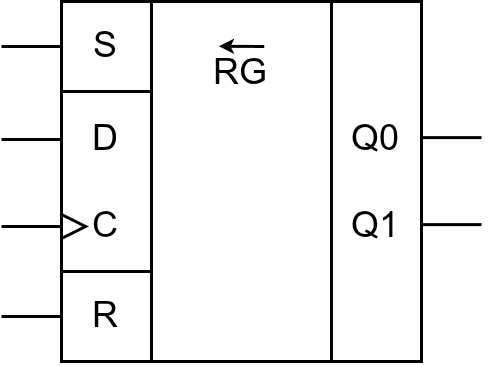
\includegraphics[width=0.4\textwidth]{pics/parzival_rg.png}
  \caption*{Рисунок 1 --- Двухразрядный сдвиговый регистр со сдвигом в сторону старших}
\end{figure}

S (Set) -- установка регистра в положение <<1>>; D -- вход данных; С -- тактовый генератор; R (Reset) -- установка регистра в положение <<0>>; Q0 и Q1 -- выходы разрядов регистра.

\section{Построим функциональную схему устройства}

\begin{figure}[H]
  \centering
  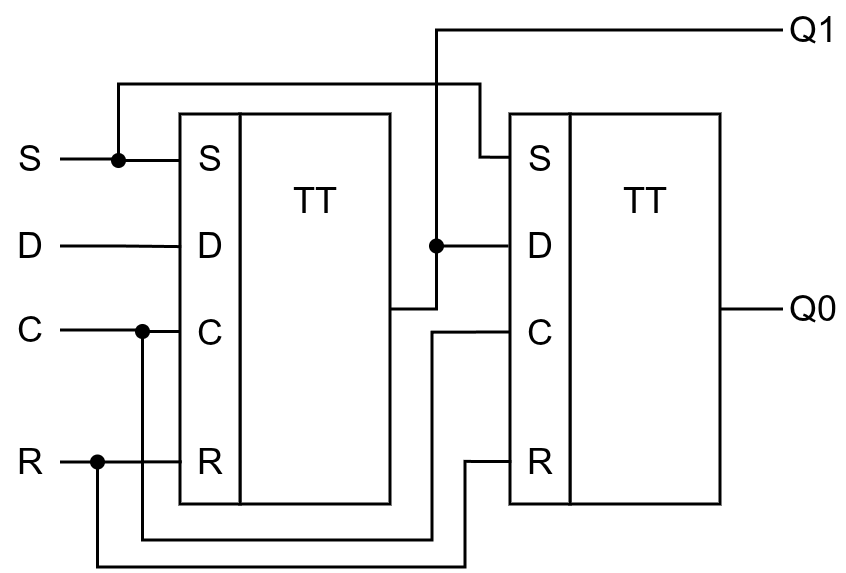
\includegraphics[width=0.9\textwidth]{pics/parzival_logic.png}
  \caption*{Рисунок 2 --- Функциональная схема устройства}
\end{figure}

\newpage
\section{Построим принципиальную схему устройства}

\begin{figure}[H]
  \centering
  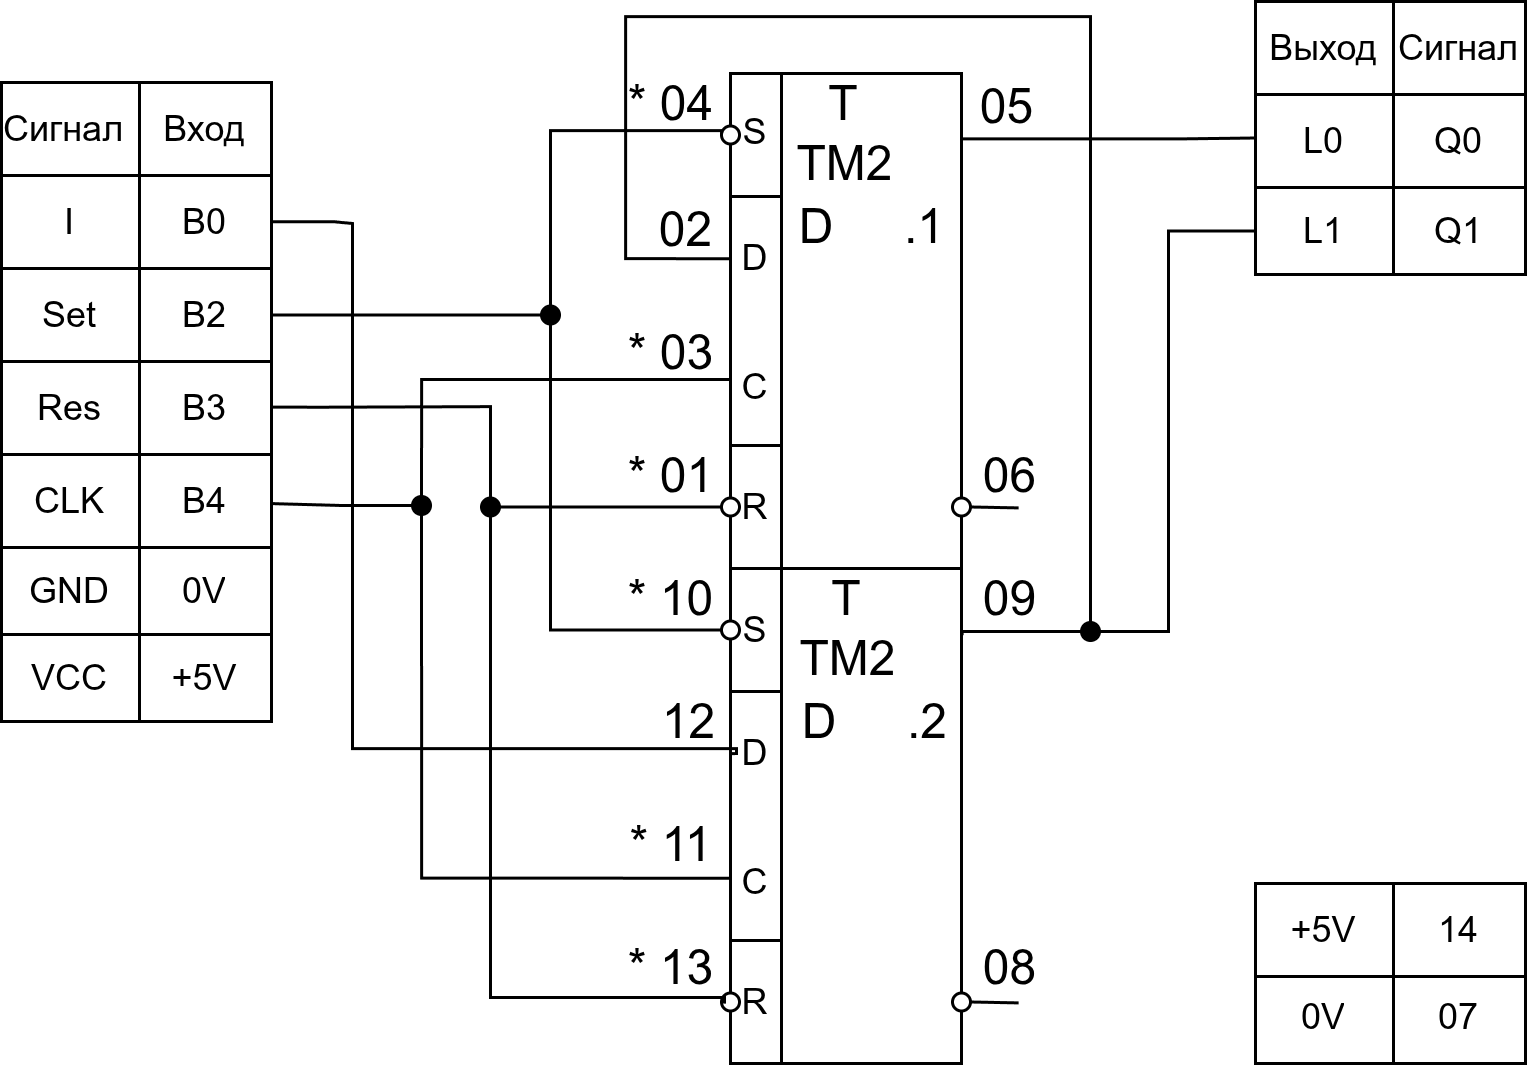
\includegraphics[width=0.9\textwidth]{pics/parzival_circuit.png}
  \caption*{Рисунок 3 --- Принципиальная схема устройства}
\end{figure}

\newpage

Определим контакты питания для микросхемы ТТЛ:
\begin{center}
  Таблица 4 --- Таблица питания для микросхем ТТЛ \\
  \vspace{5mm}
  \begin{tabular}{|c|c|c|}
    \hline
    Микросхема & +5V & 0V \\
    \hline
    D1         & 14  & 07 \\
    \hline
  \end{tabular}
\end{center}
\section*{Вывод}

В ходе данной лабораторной работы были получены навыки синтеза сдвигового регистра, монтажа и тестирования устройства. Функционирование устройства полностью соответствует заданной таблице истинности. Также была изучена работа элемента памяти ТМ2 (2 D-триггера).

\end{document}
